%-------------------------------------------------------------------------------
% File: overview.tex
%       
%
% Author: Marco Pinna
%         Created on <date>
%-------------------------------------------------------------------------------
\chapter{Overview}\label{ch:overview}
DVoting is a distributed electronic voting application that allows people to take part in a state election by going to the polling station, authenticating with personal ID and a smart-card, and expressing their vote on an electronic device in the polling booth.\\

Figure \ref{fig:high_lev_arch} show a high level view of the application.\\
When a voter enters the polling station, they authenticate and they enter the polling booth. In each polling booth there is an electronic device which is used to cast the vote. The voter authenticates with private key in the polling booth and they are presented with a web page where they can express their voting preference. The vote is sent from the polling booth to the polling station, which takes care of marking that the voter has cast their vote.\\
The vote is then forwarded to the central station, where it is stored in an encrypted database until the end of the election. The central station also takes care of counting all the votes and computing the outcome of the election.\\

\begin{figure}
    \begin{center}
        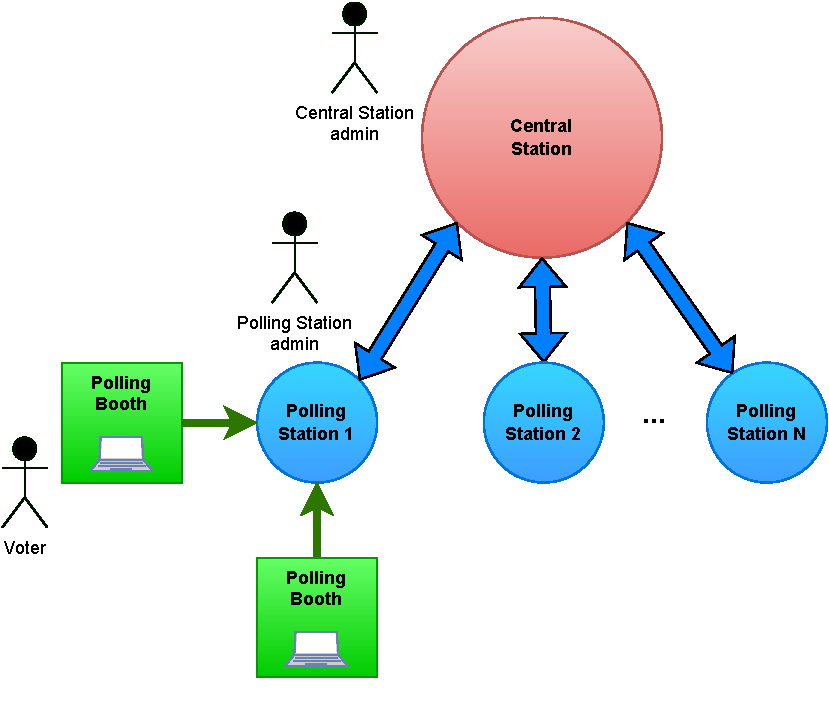
\includegraphics[scale=1]{img/high_lev_arch.pdf}
    \end{center}
    \vspace*{-0.5cm}
    \caption{High level view of the application architecture.}
    \label{fig:high_lev_arch}
\end{figure}




\section{Functional requirements}\label{sec:func_req}
The following functional requirements have been identified:

\subsection*{Voter}
\begin{itemize}
	\setlength\itemsep{1pt}
	\item An anonymous user should be able to login to the platform via private key authentication.
	\item A logged user should be able to express their voting preference via web UI on the electronic device present in the polling station.
\end{itemize}

\subsection*{Polling station admin}
\begin{itemize}
	\item An admin user should be able to login to the admin dashboard via username and password.
	\item An admin user should be able to open the vote.
	\item An admin user should be able to temporarily suspend the vote.
	\item An admin user should be able to close the vote.
	\item An admin user should be able to view statistics related to the vote such as the turnout.
	\item An admin user should be able to manually add people to the list of the voters in particular cases (military, etc.)
\end{itemize}

\subsection*{System}
\begin{itemize}
	\item The system should remember which voters already expressed a vote.
	\item The system should aggregate the votes expressed in the single polling station.
	\item The system should aggregate the total counts of vote for each candidate coming from each of the polling stations.
\end{itemize}

\section{Non-functional requirements}\label{sec:non_func_req}
The application was designed to ensure security aspects which are to be guaranteed during any election, namely:\\
\begin{itemize}
	\item Privacy and vote secrecy
	\item Double voting prevention
	\item Anonymity
	\item Authentication
	\item Authenticity
	\item Unlinkability
\end{itemize}
\hfill \break
\noindent These security aspects are achieved through the use of different means. More in detail:\\
\begin{itemize}
	\item Privacy and vote secrecy have been ensured by means of asymmetric encryption
	\item Double voting prevention is ensured by keeping track in a database of who voted and who did not.
	\item Anonymity and unlinkability are guaranteed by ``splitting" the vote and the voter identity once the former is sent to the central station
	\item Authentication is ensured by face recognition upon entering the polling station and via private key authentication.
	\item Authenticity is achieved via digital signature algorithm
\end{itemize}